\documentclass{article}
\usepackage[T2A]{fontenc}
\usepackage[russian]{babel}
\usepackage[utf8]{inputenc}

%%%%%%%%%%%%%%%%%%%%%%%%%%%% ДОП.СИМВОЛЫ  %%%%%%%%%%%%%%%%%%%%%%%%%%%%%%%%
\usepackage{amsmath}
\usepackage{amssymb}
\usepackage{latexsym}
\usepackage{amsfonts}
\usepackage{extarrows}
\usepackage{braket}
\usepackage{MnSymbol}
\usepackage{mathtools}
\usepackage{commath}

\DeclarePairedDelimiter{\ceil}{\lceil}{\rceil}
\DeclarePairedDelimiter{\floor}{\lfloor}{\rfloor}
%%%%%%%%%%%%%%%%%%%%%%%%%%%%%%%%%%%%%%%%%%%%%%%%%%%%%%%%%%%%%%%%%%%%%%%%

%%%%%%%%%%%%%%%%%%%%%%%%%%%%%  ГРАФИКА  %%%%%%%%%%%%%%%%%%%%%%%%%%%%%%%%
%Цвета:
\usepackage{color} 
\usepackage{xcolor}

%Картиночки:
\usepackage{graphicx}
\graphicspath{{pictures/}}
\DeclareGraphicsExtensions{.pdf,.png,.jpg}

%Встроенная графика 
\usepackage{tikz}
\usetikzlibrary{
    shapes.symbols,
    shapes.geometric,
    shadows,arrows.meta,
    graphs
}

\usepackage{flowchart}
%%%%%%%%%%%%%%%%%%%%%%%%%%%%%%%%%%%%%%%%%%%%%%%%%%%%%%%%%%%%%%%%%%%%%%%%

%%%%%%%%%%%%%%%%%%%%%%%%%%%%%% ВЕРСТКА 1 %%%%%%%%%%%%%%%%%%%%%%%%%%%%%%%%%
\usepackage[toc,page]{appendix}
\usepackage{hyperref}
\hypersetup{
    unicode=true,
    colorlinks=true,
    linktoc=all,  
    linkcolor=blue,
}
\usepackage{hhline}
\usepackage{subcaption}
\usepackage{float}
\usepackage{enumitem}
%%%%%%%%%%%%%%%%%%%%%%%%%%%%%%%%%%%%%%%%%%%%%%%%%%%%%%%%%%%%%%%%%%%%%%%%

%%%%%%%%%%%%%%%%%%%%%%%%%%%%%% ВЕРСТКА 2 %%%%%%%%%%%%%%%%%%%%%%%%%%%%%%%%%
% Шрифты - настройки по умолчанию.
\renewcommand{\rmdefault}{cmr}
\renewcommand{\sfdefault}{cmss}
\renewcommand{\ttdefault}{cmtt}

%Формат секции
\makeatletter
\renewcommand{\@seccntformat}[1]{}
\makeatother


%Пробел
\setlength{\parindent}{0pt}
\setlength{\parskip}{3pt}

%Размеры страницы (не забыть подогнать под принтер)
\usepackage[left=2cm,right=2cm,bottom=2cm]{geometry}

%Списки:
\setlist{topsep=1pt, itemsep=0em}
%%%%%%%%%%%%%%%%%%%%%%%%%%%%%%%%%%%%%%%%%%%%%%%%%%%%%%%%%%%%%%%%%%%%%%%%%%%%%%%%%%%%%%%%%%%%

\title{Отчет по хакатону}
\author{Stardust Crusaders}
\date{22 ноября 2020 г.}
\begin{document}
\maketitle
\tableofcontents

\section*{Резюме}

\texttt{Основной github}: \href{https://github.com/Desiment/safety-barriers}{ссылка} 

\texttt{Обработанные данные}: \href{https://drive.google.com/drive/folders/1XhPnQkAMY1KkejASQoEDTFzi1GouzvbE?usp=sharing}{ссылка} 

Написаны четыре модели, были проведены простые тесты (о каких-то статистических величинах говорить рано), построены гипотезы относительно природы данных.

\newpage
\section{Постановка задачи}
В компании вводятся так называемые “барьеры безопасности”, анализ которых сможет предотвратить негативные происшествия. Однако аналитика сопряжена с рядом проблем:
\begin{itemize}
    \item 16-20 тысяч сообщений на естественном языке в месяц. Объем регистрируемых сообщений об опасных действиях/опасных условиях с производственных площадок по компании
    \item 5 рабочих дней затрачивается на сбор обработку сообщений сотрудниками блоков и ДО. Длительный процесс не даёт возможность оперативно реагировать на сообщения о работоспособности производственных барьеров
    \item Человеческий фактор при классификации. Субъективный результат классификации сообщений и как результат – отсутствие сквозной аналитики (между ДО)
\end{itemize}

Сейчас существует цифровой проект «Определение барьеров производственной безопасности из сообщений об опасных условиях-опасных действиях».

В рамках проекта разрабатывается инструмент для классификации записей об опасных действиях и условиях, поступающих от ДО и подрядных организаций в различных информационных системах (контур безопасности, ОУ ОД БРД, АЗИМУТ и другие).

Решение позволит повысить достоверность данных, на которых принимаются решения о работоспособность барьеров и делается оценка рисков ПБ.
Появление новой аналитики позволит сфокусировать усилия сотрудников на предупреждение «пробоя» барьера промышленной безопасности.
Сократятся трудозатраты на обработку заявки и создание аналитики с 5 дней до нескольких часов.

В файле представлены данные для оценки и первичного анализа (файл мы пришлем всем командам, которые выбрали данное направление в субботу, 21 ноября после начала хакатона)
\begin{itemize}
    \item В графе place — место, где произошел прецедент промышленной безопасности
    \item В графе precedent — сам прецедент. Что такое прецедент — опасное действие, условие.
\end{itemize}

Замечания по данным:
\begin{itemize}
    \item Иногда в графу прецеденты респонденты заносят сразу несколько опасных действий и условий
    \item Данные содержат аббревиатуры, термины, неточные выражения, опечатки и сленг
\end{itemize}

Необходимо:
\begin{itemize}
    \item Построить модель кластеризации. В дальнейшем эти кластеры помогут провести аналитику для сопоставления прецедентов с классификацией опасных действий и условий — с барьерам безопасности.
    \item Объяснить получившиеся кластеры: почему они такие. Сделать вывод, можно ли с помощью них упростить какую-либо полуавтоматическую разметку данным по классам
\end{itemize}

Глобально можно выделить несколько возможных кластеров:
\begin{itemize}
    \item Прецеденты, связанные с вождением, и управлением транспортным средством (ТС)
    \item Прецеденты, связанные с использованием исправного инструмента
    \item Прецеденты, связанные с работой на высоте и с подъемом грузов
    \item Прецеденты, связанные с защитой (СИЗ (средства индивидуальной защиты), СИЗОД (средства индивидуальной защиты органов дыхания), перчатки, куртки и тп)
    \item Все остальное
\end{itemize}

\section{Используемый датасет}
Был предоставлен компанией-заказчиком.

\section{Описание решения}
\subsection{Особенности обработки данных}
Исходный \texttt{.xlsx} файл расщеплен на 5-столбцовый \texttt{.csv} файл, которые и уже обрабатывался. Дополнительно был построен словарь всех слов и словарь с подсчетом частот

\begin{figure}[h!]
    \centering
    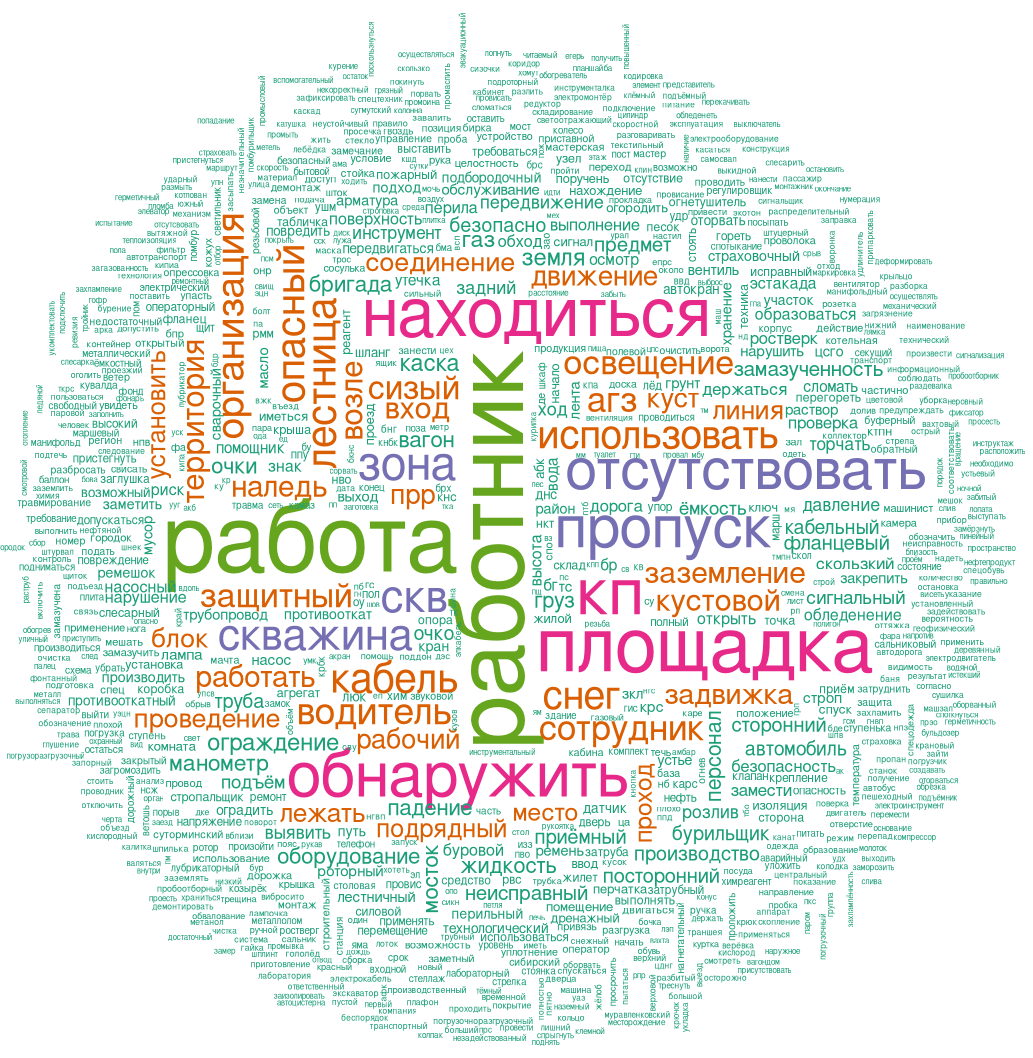
\includegraphics[scale=0.2]{image.png}
    \caption{Облако слов для очищенных данных, построенное с помощью языка R}
\end{figure}


При первичной очистке данных были удалены строчки таблицы начиная с \texttt{62000} заканчивая по \texttt{84000}, так как эти строки не соответствовали общему формату данных.

При обработке данных в первых трех моделях использовался \texttt{PyMoprhy}: в связи с чем происходила потеря значений аббревиатур и терминологии.

covid-19 встречался в сообщениях как на латинице, так и кириллице, но первый вариант так же был удален для использования \texttt{PyMoprhy}.

Для последних моделей использовался \href{http://www.tech.nftn.ru/dir/c/22}{словарь}
аббревиатур и сторонние \href{https://rusvectores.org/ru/}{специализированные корпусы}.

\newpage

\subsection{Модели}
В рамках поставленной задачи были построены 4 модели кластеризации:
\begin{itemize}
    \item Ручная кластеризация по ключевым словам;
    \item Кластеризация с помощью K-mean и Word2Vec, с использованием платформы KNIME;
    \item Кластеризация с помощью K-mean и Word2Vec, на питоне с дополнительным препроцессингом данных;
    \item Кластеризация с помощью K-mean и Word2Vec с внешним корпусом текстов и TensorFlow.
\end{itemize}

Краткое сравнение моделей

\begin{table}[h!]
    \centering
    \begin{tabular}{|c|c|c|c|c|}
    \hline
                        & Ручная кластеризация & KNIME  & Python  & Advanced  \\ \hline
    Сложность настройки & Низкая               & Низкая & Средняя & Высокая   \\ \hline
    Гибкость модели     & Низкая               & Низкая & Средняя & Высокая   \\ \hline
    Точность            & Средняя              & Высокая& Средняя & ?         \\ \hline
    Масштабируемость    & Нулевая              & Средняя& Средняя & Высокая   \\ \hline
    \end{tabular}
    \caption{Сравнение четырех моделей}
    \label{tab:my_label}
\end{table}

\subsection{Краткий обзор идей для анализа}

На текущий момент мы предложили упорядочивать данные по следующей структуре:

\begin{figure}[h!]
    \centering
    \begin{tikzpicture}[scale=0.3]
        \filldraw [fill=white, draw=black, thick] (-4,-4) rectangle (8, 8);
        \filldraw [fill=white, draw=black, thick] (-3,-3) rectangle (6, 6);
        \filldraw [fill=white, draw=black, thick] (-2,-2) rectangle (4, 4);
        \filldraw [fill=white, draw=black, thick] (-1,-1) rectangle (2, 2);
        
        \node at (0.3, 0) {msg};        
        \node at (0.3, 3) {объект};
        \node at (0.3, 4.85) {подрядчик};
        \node at (1.3, 7) {дочернее общество};
    \end{tikzpicture}
    \caption{Структура данных}
    \label{fig:structure}
\end{figure}

и исследовать особенности каждого уровня. В частности, искать сущности-\textit{аттракторы}, у которых какие-то слова или другие свойства сообщений (\texttt{msg}) встречаются чаще, чем в среднем. Так, мы искали предприятия, на которых плохо соблюдается профилактика covid-19: \texttt{grep} по строчкам очищенной таблицы содержащим слова ``ковид`` ``пандемия`` показал, что организация ``НоябрьскЭнергоНефть`` отправила большую часть сообщений с этими словами.

Полноценный поиск аттракторов не удалось выполнить. Так же, в рамках существуешь структуры данных предлагалось исследовать наличие пустых сообщений или сообщений дубликатов.

\subsection{Структура репозитория}
В корневом каталоге содержатся:
\begin{itemize}
    \item \texttt{prepare.py} --- модуль, который очищает и подготавливает данные для работы
    \item \texttt{reports/} --- каталог с отчетами и презентацией.
    \item \texttt{keywords-model/} --- каталог с моделью ручной кластеризации
    \item \texttt{word2vec-model/} --- каталог с моделями базирующихся на Word2Vec и K-means, написанных на python.
\end{itemize}

Так же есть каталог \texttt{data/} который не отображается в github`е.
В \texttt{data/} находятся следующие файлы:
\begin{itemize}
    \item \texttt{precedents.csv} --- сырые данные преобразованные в \texttt{.csv}.
    \item \texttt{fixed-precedents.csv} --- расщепленная таблица. 
    \item \texttt{documents.csv} --- таблица \texttt{fixed-precedents.csv} в которой все столбцы сведены в один для Word2Vec.
    \item \texttt{frequency.dic} --- уникальные слова в нормальной форме для поиска ключевых слов и построения облака.  
    \item \texttt{stopwords.txt} --- список стоп-слов.
\end{itemize}

На том же гугл-диске находится папка \texttt{clustering} где расположены файлы моедли KNIME. 

\section{Результаты}

Ручная модель работает исправно и позволяет делать предсказания:

\texttt{Input: "Рабочий взял оголенный электрокабель"}
\texttt{Output: "Преценденты связанные с электричеством"}

Модель на основе Word2Vec выделила много кластеров, которые требуют дополнительной обработки.

Распределение:
\begin{itemize}
    \item Ручная модель, очистка данных, отчеты - Михайлов Михаил
    \item Модель word2vec, очистка данных - Данил Ельцов
\end{itemize}



\end{document}

